\documentclass[a4paper,11pt,DIV=11]{scrartcl}
\usepackage[utf8]{inputenc}
\usepackage[version=4]{mhchem}
\usepackage[ngerman]{babel}
\usepackage{amsfonts, amsmath, amssymb}
\usepackage{graphicx}
\usepackage{float}
\parindent0pt

\title{Transmissions-Elektronen-Mikroskopie}
\author{Adrian Messow, Sven Mehrkens \\
Tutor: ???}
\date{Durchführung: 14.12.2017 \\ Abgabe: ??? }

\begin{document}
\maketitle
\section{Einführung}
In diesem Versuch werden die Grundlagen des Transmissionselektronenmikroskops (TEM) vermittelt. Dabei werden nach einer grundlegenden Justierung die Beugungsbilder im Hellfeld und Dunkelfeld an einer GaAs-Probe aufgenommen und indiziert. Durch Aufnahmen von InGaAs-Quantentrögen wird anschließend einerseits über die Intensitätsverteilung und andererseits über die Gitterkonstanten die Indiumkonzentration bestimmt.

\section{Theoretische Grundlagen}
Transmissionselektronenmikroskope erreichen eine Auflösung die im Sub-\(\mathrm{\mathring{A}}\)-Bereich liegt. Dies liegt an der Verwendung von Elektronen zur Bildgebung, anstatt von Photonen in herkömlichen Lichtmikroskopen. Dabei werden Elektronen aus einem Filament heraus beschleunigt und über Linsensysteme auf die Probenoberfläche fokussiert. Die transmittierten Elektronen werden über geeignete Beobachtungssysteme sichtbar gemacht. Das Auflösungsvermögen wird durch das Raleigh-Kriterium beschrieben und kann bei kleinen Winkelabweichungen von \(\alpha<1^\circ\) beschrieben werden durch \(\delta > 60\lambda\). Für eine typische Bechleunigungsspannung von \(100\,\mathrm{kV}\) ergibt sich zum Beispiel eine Auflösung von \(0,2\,\mathrm{nm}\). Dabei wird die Wellenlänge des Elektrons durch die \textit{de Broglie Wellenlänge} für relativistische Teilchen beschrieben: 
\begin{align}
\lambda = \frac{h}{\sqrt{2m_\mathrm{0}eV(\frac{1+eV}{2m_\mathrm{0}c^2})}}
\end{align}
Mit \(h\) dem planck'schen Wirkungsquantum, \(m_\mathrm{0}\) der Ruhemasse des Elektrons, \(c\) der Lichgeschwindigkeit und \(eV\) der Energie des Elektrons in Elektronenvolt.\\
Zwei Bildgebungsarten sich möglich. Das erste ist das Beugungsbild, hier wird das reziproke Gitter des Kristalls abgebildet. Das zweite ist das Realbild (Abb. \ref{Strahlengang}).
\begin{figure}[H]
\center
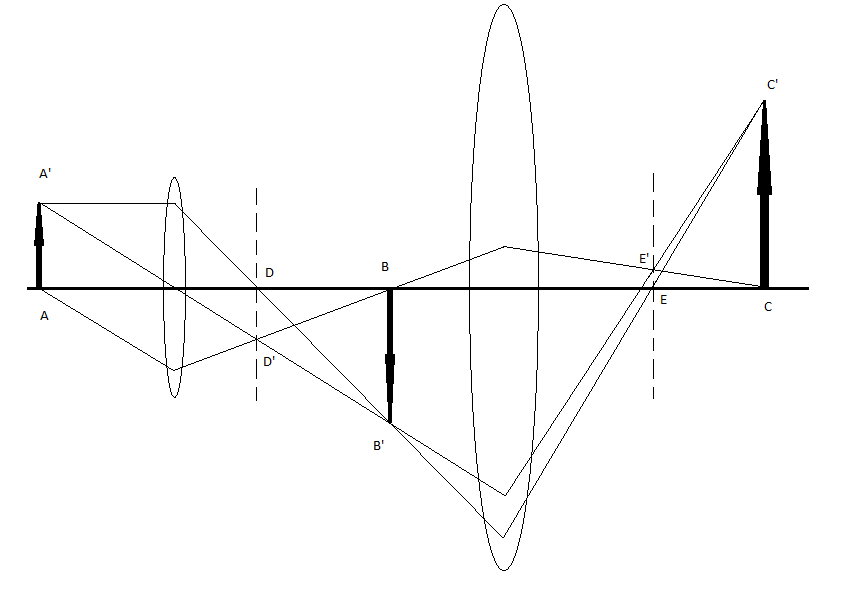
\includegraphics[width=\textwidth]{Strahlengang.png}
\caption{Schematische und vereinfachte Darstellung des Strahlenganges zur Entstehung der zwei Bildarten. Realbilder bei BB' und CC'. Beugungsbilder bei DD' und EE'.}
\label{Strahlengang}
\end{figure}
Werden Elektronen an den Atomen im Kristall gestreut, so ergibt sich eine vom Steuwinkel abhängige Intensitätsverteilung. Die Elektronen werden nach dem Bragg-Gesetz gestreut. Da die Winkel durch die kurze Wellenlänge der Elektronen jedoch sehr klein sind, kann der Bragg-Winkel genähert werden zu:
\begin{align}
2d\theta = n\lambda
\end{align}
Mit \(\lambda\) der Wellenlänge der Elektronen, \(d\) dem Abstand der Atome im Gitter und \(\theta\) dem Winkel des Elektronenstrahls zur Atomebene. Somit werden für jeden Gitterbaustein bestimmte Reflexe erwartet. Jedoch entstehen nicht von jedem Gitterbaustein Reflexe. Über den Strukturfaktor können nun die verbotenen und erlaubten Reflexe, berechnet werden.
\begin{align}
F_\mathrm{hkl}= \sum_{j=1}^n f_\mathrm{j}(\theta)\exp[-2\pi i (hu_\mathrm{j}+kv_\mathrm{j}+lw_\mathrm{j})]
\end{align}
Mit \(h,k,l\) den Millerschen Indizes, \(f_\mathrm{j}(\theta)\) dem Streufaktor und \(j=1,2,3,...,n\) dem \(j\)ten Atom in der Einheitszelle am Ort \((u,v,w)\).\\
Das Ergebnis sind Beugungsbilder, die von der Kristallstruktur abhängig sind. Besteht eine Probe aus mehreren Kristallen mit unterschiedlicher Orientierung zueinander, so überlagern sich die jeweiligen Beugungsbilder.
Eine anschauliche Verdeutlichung des Bragg-Gesetzes ist die Ewald-Kugel. Dabei wird in das reziproke Gitter des Kristalls der einfallende Elektronenstrahl mit der Länge \(1/\lambda\) auf einen gewählten Ursprungsreflex gezeichnet. Die Länge des Elektronenstrahls gibt den Radius eines Kreises, dessen Mittelpunkt der Anfang des Elektronenstrahls definiert. Alle Reflexe, die nun auf dem Kreis liegen, sind im Beugungsbild erkennbar. Da die Intensitätsbreite des Bragg-Winkels von der Dicke der Probe mit \(1/t\) abhängt, weicht das reziproke Gitter auf und es sind keine Punkte mehr, sondern Linien. Somit sind auch Relfexe sichtbar, wenn die Ewaldkugel knapp die Reflexe verfehlt. 
	
\section{Versuchsaufbau und Versuchsdurchführung}

\section{Auswertung}

\section{Zusammenfassung}

\section*{Anhang}

\end{document}